\chapter{绪论}
%
\section{RISC指令集架构与RISC-V}
\subsection{研究背景}

指令集架构(Instruction Set Architecture,ISA)是计算机体系结构中,介于微处理器架构(Microarchitecture)与操作系统之间的接口。指令集架构用于抽象微处理器底层的具体硬件实现以提供给操作系统一个简洁的硬件接口来管理计算机硬件系统。最早的指令集架构可以追溯到1964年IBM发布的IBM System/360指令集架构,并实现在同时发布的IBM 360计算机族当中[1]。IBM System/360的设计初衷是为了给IBM 360计算机族中不同型号的微处理器为操作系统提供一个统一的接口,而无需针对不同的微处理器实现而设计不同的接口。

指令集架构经过几十年的发展,现今已经出现了众多主流的指令集架构。下面对最为流行的三种指令集架构进行介绍:

\begin{enumerate}
	\item 	x86。x86是1978年由Intel公司推出的著名复杂指令集计算机(Complex Instruction Set Computer,CISC)指令集架构,作为桌面型个人计算机市场最主流的指令集架构,其成功来源于推出时对IBM计算机的兼容以及较好的向后兼容性。然而,从现今的眼光看来,x86已经变得臃肿而复杂,自发展至今到现在x86已经添加了大量的复杂指令。截止2015年,x86已经拥有1300多条指令,大量的寻址模式,大量的特殊寄存器以及多种转换寻址的策略。同时,x86也有一些固有的缺陷,如贫瘠的寄存器数目以及多种隐式的技术特性,包括隐式的条件编码以及预测移动等,这在高性能的微处理器中是难以实现的[2]。
	\item	ARM。ARM是1985年由ARM Holding公司开发的精简指令集计算机(Reduce Instruction Set Computer,RISC)指令集架构。ARMv7是ARM的32位版本,2011年发布了基于64位的ARMv8版本。ARM由于其低功耗、低成本的特性,被广泛应用于嵌入式系统当中。在RISC-V发布前,ARM在嵌入式市场占据绝对主导地位,且在大多数的消费电子设备如便携式设备以及电脑外设等当中占有大部分的市场。然而,ARM也存在着不少的缺点,如混合的特权级以及用户级架构、独立的压缩指令集Thumb等。
	\item	MIPS。MIPS是1985年由MIPS科技公司开发的RISC指令集架构。MIPS是最经典的RISC架构,其影响了后续大多数的RISC指令集架构的设计思想。MIPS采用加载-存储的存储器访问架构,这意味着只有加载以及存储两种内存指令,其他所有的算术操作都是在寄存器上进行,这种设计降低了指令集以及实现硬件的复杂性,在编译器技术提升的基础上,可以促进更为简单的流水线处理器实现。虽然MIPS简单易行设计使得在学术领域青睐有加,但是该指令集架构还是有几个技术上的缺陷使得它对于高性能的实现来说不具有吸引力,如固定的分支延迟间隙(Delay Slot)、对动态链接的支持非常糟糕、乘除法使用了特殊的架构寄存器等等。
\end{enumerate}

从上述三个典型的主流指令集的现状可以看出,目前的指令集架构发展趋势主要有以下方面:

\begin{enumerate}
	\item RISC指令集占据主导地位。进入21世纪以来,仍在广泛流行的CISC指令集仅剩下x86。同时,随着AMD K2微处理器架构发布以来,所有的Intel的乱序执行的处理器引擎都会动态的将x86的指令转化成内部的更接近于RISC风格的微指令执行。x86芯片的出货量自2011年达到峰值以来,每年下降近10%,而采用RISC处理器的芯片出货量则飙升至200亿。
	\item 主流指令集架构囿于设计年代久远而逐渐暴露历史遗留缺陷。x86随时间不断膨胀而变得臃肿的指令集,ARM低效的压缩指令集Thumb,MIPS固有的分支延迟间隙,这都是在当初指令集设计之初并没有预料到的缺点,伴随着异构体系结构的兴起,年迈的ARM以及MIPS在对现代高性能的微处理器设计中已经显得逐渐力不从心。
	\item 开源、免费的指令集架构兴起。x86以及ARM是闭源的指令集架构,闭源的指令集架构会阻碍成功的学术成果在商业化道路上的发展。如果想要设计一款基于上述指令集的微处理器,则需要缴纳大笔的授权费用。MIPS面对RISC-V的推广后也宣布为开源指令集架构,在此之前MIPS同样受到知识产权的保护。免费开源的指令集架构意味着任何个人或者团体都可以基于该指令集设计微处理器,并自行决定开源亦或者是闭源该处理器实现。
\end{enumerate}

为了解决上述的问题,伯克利大学在2010年启动了RISC第五代项目计划,开发了新一代的RISC指令集架构:RISC-V。RISC-V吸取了上述提到了RISC指令集使用以及开发过程的经验,且在设计过程中匹配了现代计算设备的性能与功耗需求,其主要特点包括有:

\begin{enumerate}
	\item 将指令集划分为一个小型的基本指令集以及若干个可选的扩展指令集。RISC-V包含32位以及64位的指令集系统。以32位指令集为例子,RISC-V规定32位整型指令集(RV32I)为基本指令集架构,即所有基于RISC-V实现的32位微处理器都必须实现RV32I指令集。从另一方面来说,一个仅实现了RV32I指令集的微处理器,在不考虑性能的情况下,都可以执行任意的编译为RISC-V的程序。而根据微处理器面向的场景与功能需求,可以实现额外的扩展指令集,如乘除指令集(M)、压缩指令集(C)等等。目前,RV32I以及RV64I指令集都已经处于冻结的状态,在未来也不会发生任何改变,这种模块化的设计吸取了x86的教训,为了保持二进制代码的向后兼容性,同时维持基本指令集的简洁不变,所有新加入的指令将会以扩展指令集的方式存在[3]。
	\item 指令集架构与具体微处理器架构的严格分离。对于指令集架构的设计者来说,在指令集当中对于特定微处理器实现添加某条指令会对性能以及成本带来提升,但是却对其他的实现或者未来的实现带来负担。以MIPS的分支延迟间隙为例子,该设计为了优化早期的MIPS流水线设计中的分支指令所带来的性能损耗问题,而定义为分支的操作固定在分支指令的下一条指令执行完后再执行,而程序员/编译器则需要往这一间隙中填充有用的指令即可。然而,这种设计对于后来更深的MIPS流水线设计以及更先进的分支预测策略来说成为了一种累赘,使用MIPS实现的微处理器为了保证指令集的向后兼容性,需要花费大量的时间适配该行为。RISC-V为了避免这种情况的发生,在指令集设计过程中避免了对微处理器架构的过多设计,保持从低功耗的嵌入式微处理器到大型数据仓库式微处理器的一致性。
	\item 开源指令集。RISC-V属于一个开放的非盈利性质的基金会,其不受任何一个公司的兴起或者没落所影响。RISC-V指令集可以供任何个人或者团体免费使用,包括开发基于RISC-V的芯片或者软件,而不需要支付任何授权的费用。这对于工业界来说RISC-V是一大优势,通过复用开源的基于RISC-V的IP软核设计,可以极大的降低微处理器实现的门槛。同时,对于学术界的基于RISC-V的微处理器实现也可以平稳的转移到商用微处理器上。
\end{enumerate}

此外,RISC-V还具有其他的特性,如适配从袖珍的低功耗嵌入式微处理器到高性能计算机等各种规模的处理器;适配所有的芯片后端工艺,包括现场可编程逻辑门阵列(FPGA)以及专用集成电路(ASIC);适配所有的微架构,包括顺序执行与乱序执行的流水线、单发射或超标量的流水线;支持异构体系结构,包括领域专用的加速器实现等等。基于以上的特性,RISC-V现今在学术界以及工业界都吸引了极大的关注,近年来涌现了大量基于RISC-V的微处理器实现,本文将挑选数个典型的基于RISC-V的微处理器实现进行简要介绍。

\subsection{国内外研究现状}

本节将会对数款现今国内外主流的开源RISC-V微处理器进行简要的介绍。目前,国内外开源的RISC-V微处理器实现种类繁多,从低功耗的嵌入式微处理器到高性能的桌面型计算机处理器都有相应的开源实现。

Rocket[4]是RISC-V基金会开发的标准RISC-V微处理器实现之一,使用Chisel硬件构造语言进行设计。Rocket是一个5级的顺序单发射流水线处理器,通过配置可以实现为RV32G或RV64G内核,这两者的区别仅为使用不同的地址总线宽度以及增加了相应的双字操作。Rocket Core包括有一个内存管理单元(MMU)来支持基于页级的虚拟内存实现,一个非阻塞的数据缓存以及一个包含分支地址预测的处理器前端。分支地址预测器的参数可以进行配置,其通过分支目标缓存(BTB)、分支历史表(BHT)以及返回地址栈(RAS)来实现。对于浮点实现,Rocket Core直接复用了Chisel的标准浮点单元库进行实现。Rocket Core还支持三级特权架构:机器级、特权级以及用户级。同时,Rocket Core 还开放了一系列的参数供用户配置生成不同大小的内核,包括对M、A、F、D扩展指令集的实现、浮点流水线的级数以及缓存和TLB的大小等。Rocket的流水线结构如图1-1所示:

\begin{figure}[htbp]
	\centering
	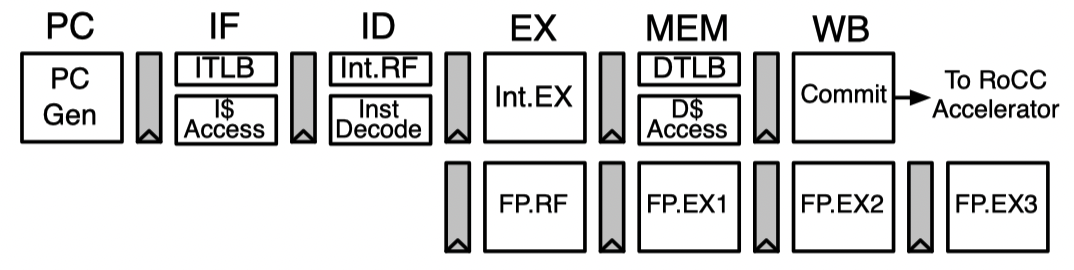
\includegraphics[width=0.95\textwidth]{Photos/Rocket_Pipeline.png}
	\caption{Rocket的流水线结构}
\end{figure}

Rocket面向的应用场景为低功耗优化下的高性能嵌入式设备,在同等TSMC 40nm工艺条件下,相比起对标的ARM Cortex-A5微处理器,Rocket具有相近的性能表现以及更小的面积以及更低的功耗:Dhrystone评分A5为1.57,Rocket为1.72(单位为:DMIPS/MHz)。面积上A5为0.53$mm^2$,Rocket为0.39$mm^2$。动态功耗上A5小于0.08mW/MHz,Rocket为0.034mW/MHz。

BOOM[5]是RISC-V基金会开发的另一个标准RISC-V微处理器实现。与Rocket不同,BOOM采用的是超标量乱序执行流水线实现,支持指令集为RV64G。与Rocket相同,BOOM也使用Chisel进行设计实现,因此在BOOM当中复用了大量Rocket中实现的模块生成器代码。BOOM很大程度上受到MIPS R10000[6]以及Alpha 21264[7]实现的启发,与这两种实现相同,SonicBOOM实现采用了显式寄存器重命名[8]的技术。BOOM的流水线结构如图1-2所示,BOOM采用了10级流水线结构,译码阶段采用4路译码,乱序执行算法在Tomasulo算法基础上加入重排序缓冲区技术改进,使指令最终提交时维持发射顺序,以达到维护精确中断的效果。

\begin{figure}[htbp]
	\centering
	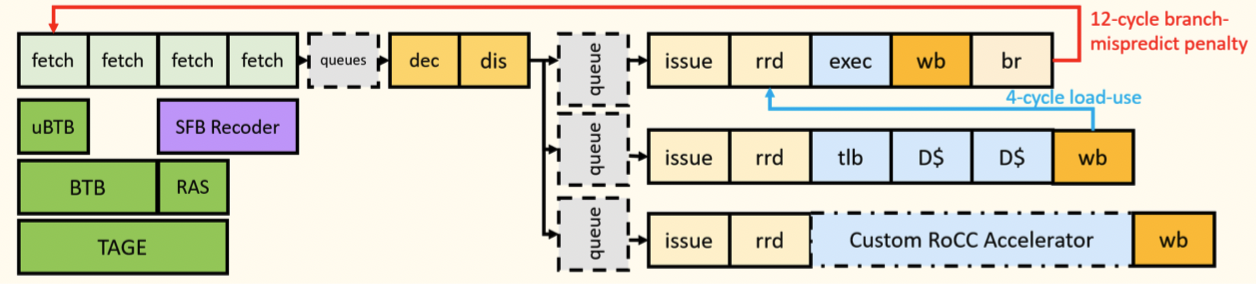
\includegraphics[width=0.95\textwidth]{Photos/BOOM_Pipeline.png}
	\caption{BOOM的流水线结构}
\end{figure}

BOOM面向的应用场景为兼具高性能以及高能效的消费类移动端/网络设备,在同等TSMC 40nm工艺条件下,相比起对标的ARM Cortex-A9微处理器,BOOM具有稍好的性能表现,同时具有更小的面积以及更低的功耗:CoreMark评分A9为3.59,BOOM为3.91(单位为CoreMarks/MHz)。面积上A9约为2.5$mm^2$,BOOM约为1.00$mm^2$。功耗上A9为0.5-1.9W,工作主频为0.8-2.0 GHz,BOOM为0.25W,工作主频为1 GHz。

Hummingbirdv2 E203[9]是国内芯来公司所研发的面向超低功耗及面积优化的嵌入式设备RISC-V微处理器,支持RV32IMAC以及RV32EMAC指令集,两级顺序执行流水线结构,且仅实现了机器级特权模式。E203的主要亮点在于其可配置的NICE(Nuclei Instruction Co-unit Extension)系统,可以允许用户自定义指令,在保持低功耗的前提下提升与外部领域专用加速器交互的性能。E203的SoC架构如图1-3所示。

\begin{figure}[htbp]
	\centering
	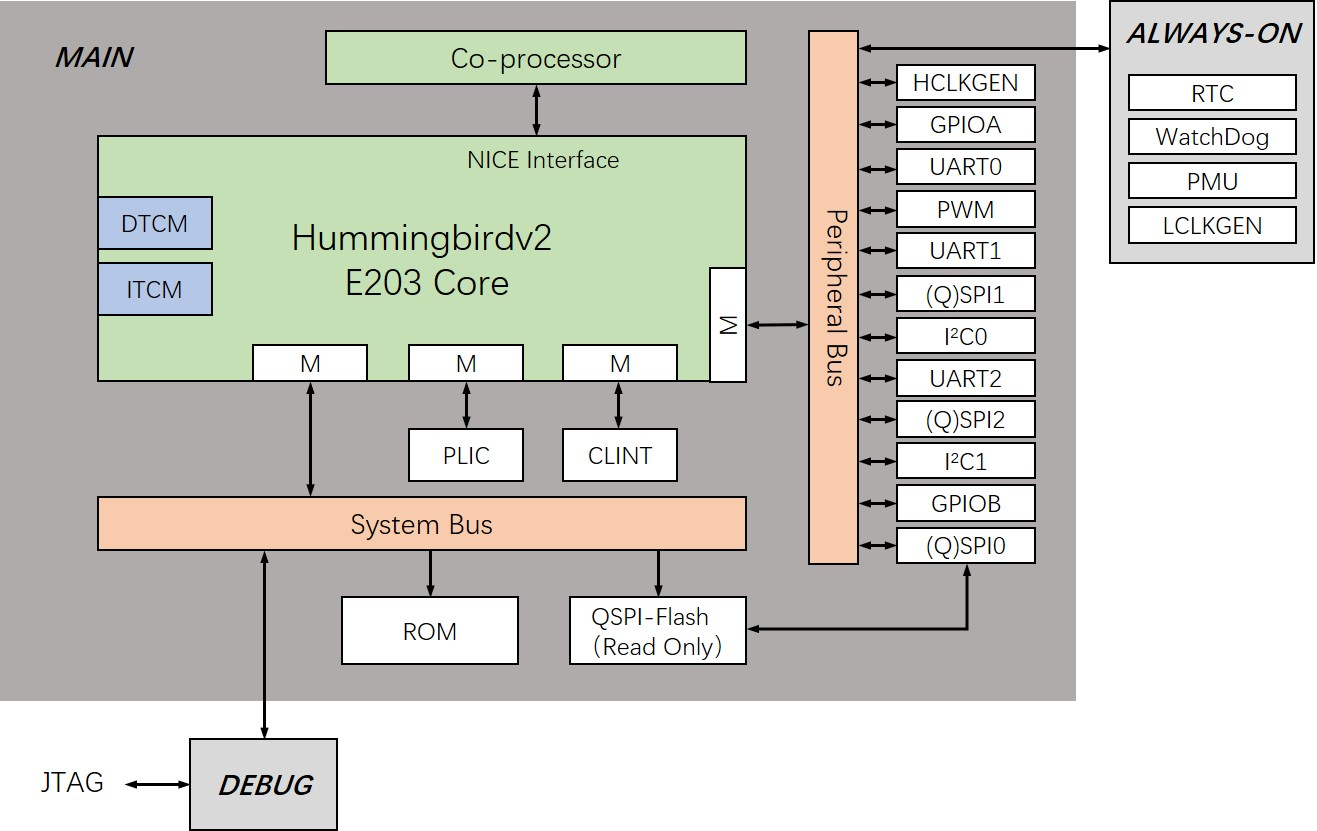
\includegraphics[width=0.95\textwidth]{Photos/hbirdv2_soc.jpeg}
	\caption{E203 SoC架构图}
\end{figure}

E203与其对标的ARM Cortex-M0/M0+相比,在维持相近的逻辑门数量前提下,能够达到更优的性能表现,且包含了多周期的硬件乘法与除法器:Dhrystone Cortex-M0与M0+的分数分别为0.84与0.93,而E203为1.23(单位:DMIPS/MHZ)。CoreMark Cortex-M0与M0+的分数分别为1.62与1.77,而E203为2.15(单位:CoreMarks/MHz)。三者逻辑门的数量都为12K。

PicoRV32[10]是由Clifford Wolf专为FPGA平台设计的面积深度优化的RISC-V微处理器实现。PicoRV32可以配置为支持RV32E,RV32I,RV32IC,RV32IM以及RV32IMC指令集的内核,同时带有一个可选的内置中断控制器。PicoRV32在Xilinx 7-Series FPGA开发板上仅占用750-2000 LUTs,且能够达到250-450MHz的工作频率。鉴于其优秀的性能与面积以及可选的协处理器接口,可以很容易的将一些针对FPGA的特定应用协处理器(音视频加速器、神经网络加速器)等移植到包含PicoRV32的FPGA系统上。

RI5CY[11]微处理器项目是瑞士苏黎世联邦理工大学(ETH Zürich)的综合系统实验室(IIS:Integrated Systems laboratory)和意大利博洛尼亚大学(University of Bologna)的高能效嵌入式研究组(EEES:Energy-efficient Embedded Systems)联合设计研发的PULP[12](Parallel Ultra-Low Power)项目中的其中一个子项目。PULP的目的是实现一个开放、可扩展的SoC,其包含的子项目如图1-4所示。其主要目的是解决IoT设备中日益增长的大量运算负载的场景。PULP支持多种处理器核架构,RI5CY是其中的一种处理器核实现。RI5CY是一款4级流水线的32位RISC-V微处理器,其包含了RV32IMC以及可选的“F”单精度浮点数扩展指令集实现。同时,为了提高DSP处理性能,RI5CY还包括自定义指令集如硬件循环(Hardware Loop)、乘累加(MAC)指令以及向量操作指令等。目前RI5CY项目已经迭代为CV32E40P[13]微处理器项目,在RI5CY的项目基础上添加了对标准RISC-V核内本地中断控制器以及高级调试模式的支持。

\begin{figure}[htbp]
	\centering
	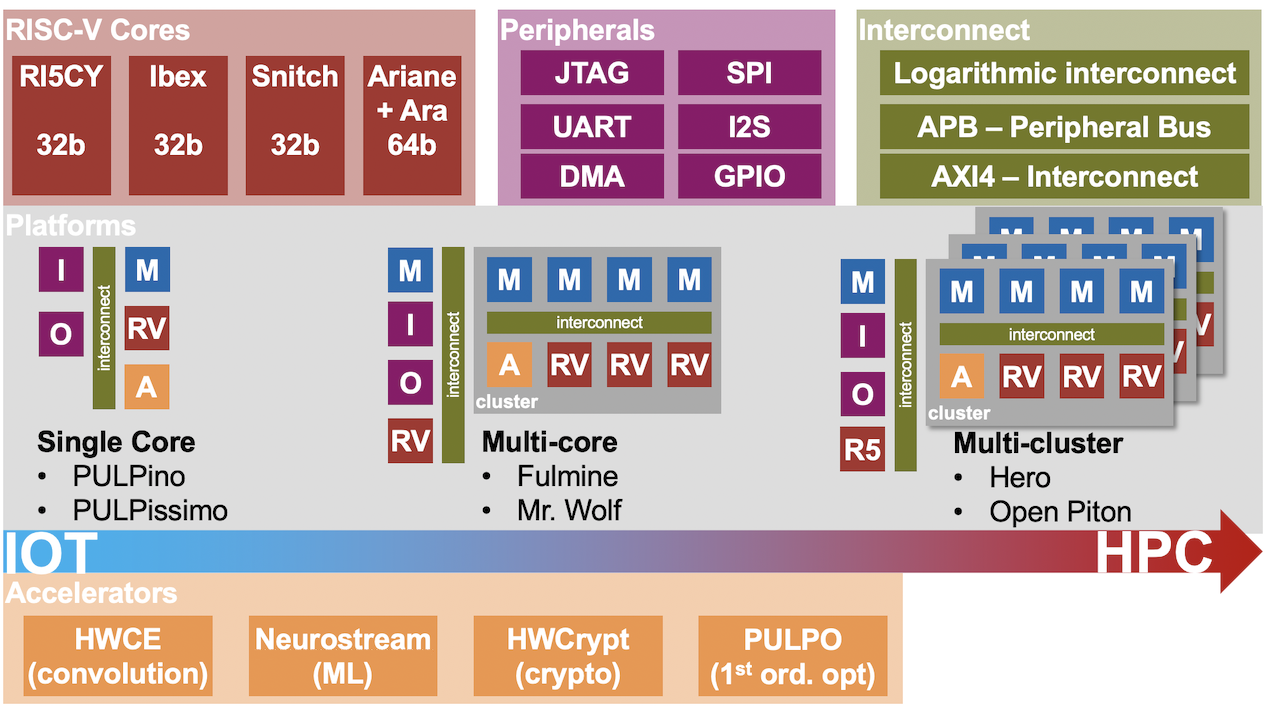
\includegraphics[width=0.95\textwidth]{Photos/pulp_family.png}
	\caption{PULP项目平台概览}
\end{figure}

RI5CY在性能上与其对标的Cortex-M4微处理器基本持平,在面积以及动态功耗上都要优于Cortex-M4:CoreMark Cortex-M4的分数为3.40,而RI5CY为3.19(单位:CoreMarks/MHz)。在65ns的工艺下,Cortex-M4的动态功耗以及面积分别为23.2µW/MHz、0.062$mm^2$,而RI5CY则分别为17.5µW/MHz、0.050$mm^2$。

香山[14, 15]是由中国科学院计算技术研究所在2021年发布的一款开源高性能RISC-V处理器,使用了包括Chisel、Verilator、GTKwave 等在内的大量开源工具,实现了差分验证、仿真快照、RISC-V 检查点等处理器开发的基础工具,建立起了一套包含设计、实现、验证等在内的基于全开源工具的处理器敏捷开发流程。香山处理器实现了RV64GC指令集,采用乱序六发射结构设计,前端包括取指单元、分支预测单元、指令缓冲等单元,顺序取指。后端包括译码、重命名、重定序缓冲、保留站、整型/浮点寄存器堆、整型/浮点运算单元。香山处理器使用了分支预测器向前覆盖的机制来实现分支预测策略,主要目的在于使用使用容量大、预测算法更复杂、得到指令信息越多的预测器来保证更高的预测准确率,但缺点在于预测器得出结果的延迟比较高,因此香山还使用了一些小型的预测器进行先行预测。香山处理器的架构如图1-5所示。

\begin{figure}[htbp]
	\centering
	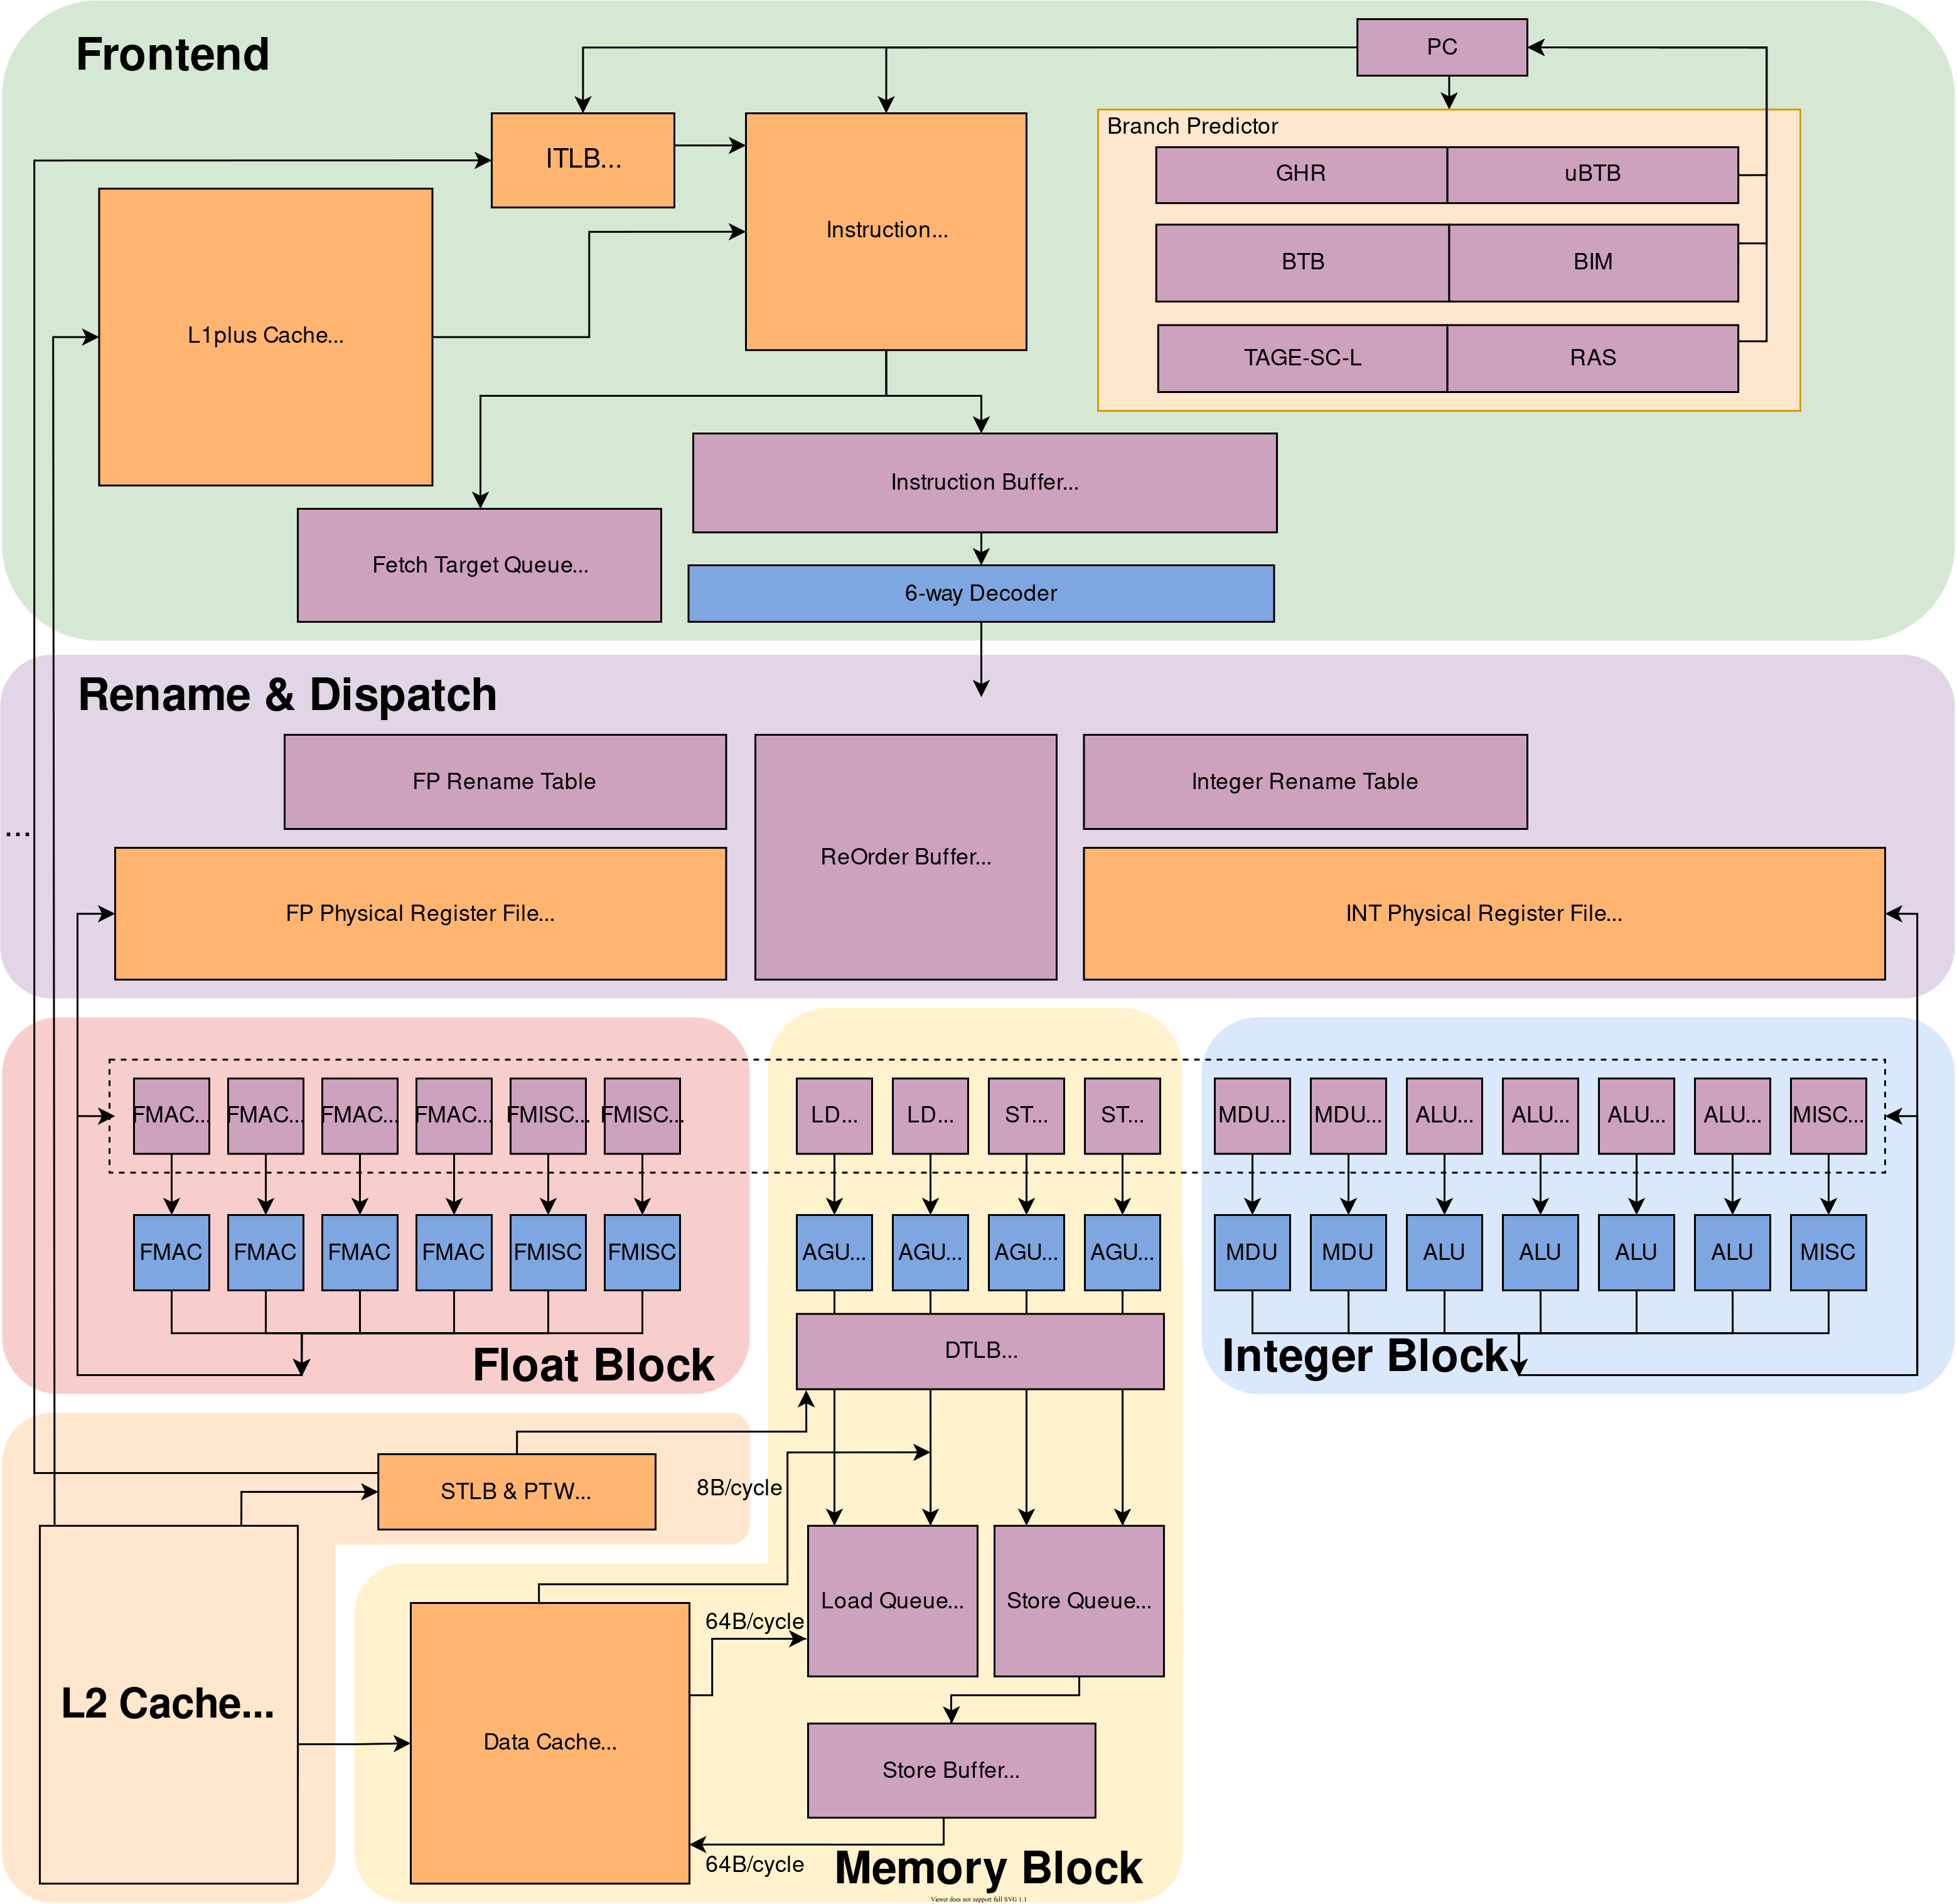
\includegraphics[width=0.95\textwidth]{Photos/xs-arch-simple.png}
	\caption{香山处理器架构图}
\end{figure}

香山处理器具有不俗的性能表现,香山的第一版架构“雁栖湖”在28nm工艺的频率上能够达到1.3GHz的频率。而目前正在开发的第二版架构“南湖”则在14nm工艺上能够达到2GHz的频率。并且,香山处理器目前已经在FPGA部署上启动了Linux/Debian操作系统,成为第一个国内完全开源的支持UNIX系统的微处理器。

\section{硬件设计方法学概论}
\subsection{研究背景}

囿于丹纳德缩放定律以及摩尔定律的终结,现今计算机体系结构面临着数个显著的挑战。丹纳德缩放定律的失效使得功耗变为现今集成电路设计的首要关键因素,而摩尔定律的终结则减缓了对晶体管技术的进步。因此,计算机架构师必须要寻找其他的途径来提高计算机系统的整体性能,这其中的重要策略之一则是使用领域特定架构(Domain Specific Architecture,DSA),也就是所谓的加速器来构成异构的计算机系统。然而,传统的硬件开发方法论缺乏在进行异构系统的设计时,缺乏相应的生产力以及效率。在过去的数十年中,瀑布模型一直是硬件开发流程所使用的设计模式,如图1-6所示。在瀑布模型的设计模式当中,开发者必须在当前阶段全部完成后才能够进入下一个阶段。举例来说,开发者只有对当前芯片所有功能的RTL设计完成后,才能够进入前端验证的阶段。如果在任意一个阶段中发现问题,则需要放弃该阶段中所有已经完成的工作而回退到上一阶段重新进行设计,且越进行到后续的阶段,解决问题的成本将会指数型的上升。

\begin{figure}[htbp]
	\centering
	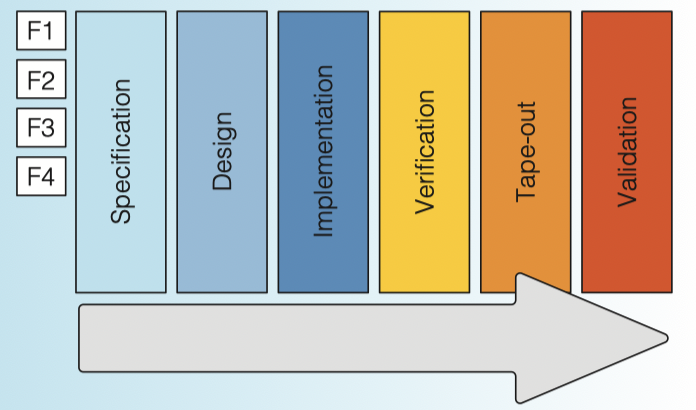
\includegraphics[width=0.95\textwidth]{Photos/waterfall.png}
	\caption{硬件开发流程中简易的瀑布模型示意,F1~F4表示了该设计的功能单元。从左到右的阶段分别为设计需求分析、架构设计、(RTL)实现、验证、流片、样片功能测试。可以发现瀑布模型中设计所有的功能单元完成当前阶段的开发后才能进入下一个阶段。实际开发流程中每个阶段都包含了相当多的具体步骤。}
\end{figure}

为了解决这个问题,伯克利大学的计算机体系结构研究团队(BAR)提出了硬件敏捷设计的方法学[16]。硬件敏捷设计的主要思想是通过快速迭代开发不完全功能的原型系统来达到敏捷设计的效果。举例来说,对于一个基于RV32G指令集微处理器的实现,硬件敏捷设计方法通过快速开发一个仅支持RV32I的芯片原型并进行流片,以获得在当前工艺下原型设计的具体参数,并以此为基础修正原先的设计。在此基础上,再添加乘除法、浮点等功能单元,并最终迭代得到成品。在硬件敏捷开发的设计模式下,当功能A进入下一阶段时,负责当前阶段的团队可以立即着手对功能B的开发。硬件敏捷开发的设计模式如图1-7所示。

\begin{figure}[htbp]
	\centering
	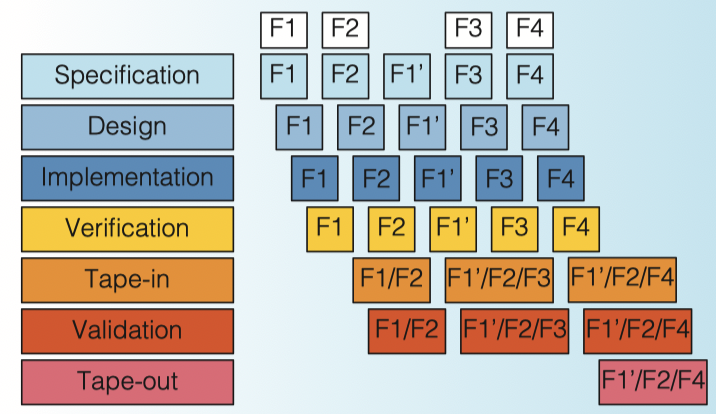
\includegraphics[width=0.95\textwidth]{Photos/agile_hardware_dev.png}
	\caption{硬件敏捷开发设计模式示意图}
\end{figure}

为了在硬件开发中引入敏捷设计模式,还需要对硬件设计工具以及框架进行改进,传统的Verilog/SystemVerilog语言无法匹配敏捷设计的需求,因此,近几年来大量基于高层次语言的硬件生成框架(Hardware Generation Frameworks,HGFs)应运而生。除了通过引入敏捷设计模式来提高硬件开发的效率,还有一种可以显著加速异构计算体系设计的方法:通过高层次综合(High-Level Synthesis,HLS)[17]的方法设计加速器。HLS允许用户将所需要实现的加速器算法以特定的C/C++语言描述出来,并通过专用的编译器生成优化过的Verilog代码。然而HLS对于架构师来说具有相当曲折的设计曲线,且目前HLS的设计优化仍然主要依赖于经验。因此,本文将重点主要放在基于高层次语言的硬件生成框架/语言当中,下一节将会介绍目前国内外对基于高层次语言的敏捷设计驱动的硬件生成框架/语言进行介绍。

\subsection{国内外研究现状}

早期对于硬件生成框架的研究项目有Verischemelog[18],它将Verilog语言混入Scheme[19]语言当中来描述硬件结构。早期的硬件生成框架项目还有Genesis2[20],它与Verischemelog的思路类似,但Genesis2是将Verilog语言混入到Perl语言当中。早期的硬件生成框架的设计都比较粗糙,一般仅使用字符串处理的方法来生成设计的Verilog代码,整体的编译过程都是静态的。因此,这些架构都缺乏可扩展性以及灵活性。

Chisel[21]是现代硬件生成框架的先驱,其作为RISC-V的衍生项目而诞生。Chisel并非简单的使用字符串处理的方式来将Verilog语言混入到某种高级语言当中,而是基于Scala[22]开发了一个完整的硬件开发库,其中包含了小到描述线网、寄存器、存储器、逻辑门的原语,大到算术逻辑单元、控制器、DSP的生成器。同时,Chisel还包含了一个介于Chisel以及Verilog之间的中间语言层FIRRTL[23, 24],它本质上是一个高度抽象化的RTL级语言。由于Chisel本质上属于使用Scala开发的第三方库,因此使用Chisel进行RTL级的硬件描述,并且支持Scala所有的语言特性,包括参数化、面向对象编程、函数式编程等等,这些特性在硬件敏捷开发模式当中将起到关键的作用。截至目前,已经有多个使用Chisel开发的微处理器、SoC以及加速器项目,如上面提到的Rocket、BOOM以及Raven-3[25]、FireSim[26]、ChipYard[27]等等。然而,Chisel在验证方面并没有给出比较完善的解决方案。目前Chisel仅支持使用基于Chiseltest[28]的单元测试验证方法,并不支持对于基于大规模的功能测试、系统测试的UVM验证方法学。Chisel整体的框架如图1-8所示。

\begin{figure}[htbp]
	\centering
	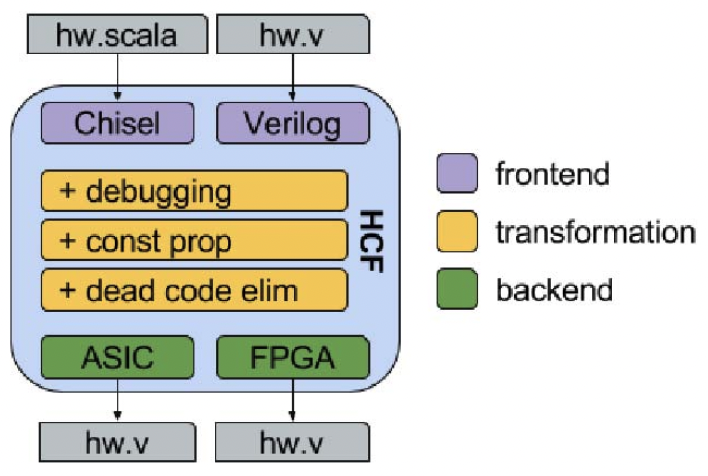
\includegraphics[width=0.95\textwidth]{Photos/chisel.png}
	\caption{Chisel整体框架图}
\end{figure}

与Chisel类似,使用Scala作为高层语言宿主的硬件生成框架还有SpinalHDL[29]。SpinalHDL最初是为了解决Chisel所缺乏的多时钟域功能所诞生的衍生性项目。与Chisel不同,SpinalHDL在设计之初采用更偏向于实际工程开发的风格,支持常见的EDA工具链。SpinalHDL不具有FIRRTL中间层,而是从Scala直接编译为对应的Verilog代码,且编译过程中不存在黑盒机制。并且,SpinalHDL不会带来额外的面积或者性能上的开销。因此,SpinalHDL相对于Chisel要更受工业界的欢迎,而Chisel则普遍受众于学术界研究。

相比较于近年来才开始流行基于Scala的硬件生成框架,基于Python的HGF设计在世纪初就开始有项目进行尝试。PyHDL[30]是最初较为流行的基于Python的脚本式硬件描述语言,它使用PamDC以及PAM-Blox两个C++硬件设计库扩展Python语言,其中,PamDC提供了硬件描述语言所需要的原语如寄存器以及线网,而PAM-Blox则是使用PamDC原语构造的工具集,包含了参数化以及面向对象的硬件模块。MyHDL[31]是一个免费开源的用于硬件描述以及验证的Python库。MyHDL将Python代码编译为Verilog或者VHDL并提供基于Python的设计代码与主流EDA工具交互的方法。MyHDL包含一个运行在Python解释器顶层的仿真器,并使用PLI(Procedural Language Interface)来与仿真器进行交互。然而,基于Python的仿真器在性能上存在劣势,并且MyHDL并不支持基于UVM的验证方法。Stratus[32]是一个基于Python的超大规模集成电路(Very Large Scale Integration,VLSI)描述语言,Stratus通过一系列的方法以及函数对Python进行扩展,来生成VLSI设计的线网(Netlist)模型。PHDL[33]同样使用Python作为硬件描述的语言,其主要亮点在于包含一个内置的模块库用于微处理器设计。然而PHDL不包含任何验证的工具或方法,仅提供了针对微处理器开发的设计模式。Migen[34]与Stratus类似,也是基于Python的VLSI设计工具,Migen基于硬件描述语言FHDL,它包含了一个形式化描述的系统来描述电路中的组合电路信号或时序电路状态。同样,Migen仅仅专注于对系统的描述,而缺乏对所设计电路的验证方法。PyRTL[35]是一个新兴的基于Python的开源硬件设计语言,与Chisel类似,它主要的设计目标在于快速的硬件原型构建。PyRTL与PyHCL一样,都是为了达到对硬件描述的简洁化。然而,PyRTL依然缺乏对设计的验证方法或工具,仅提供了一个效率低下的内置仿真器。PyMTL[36]及其后代版本Mamba[37]是一个基于Python的多层次的硬件建模工具, 它的主要特点在于使用的是在三种层次:功能级(Functional Level)

时钟周期级(Cycle Level)以及RTL级上的建模。PyMTL提供了基于PyPy JIT(即时编译)解释器的仿真器,然而其效率相比业界基于C/C++的开源仿真器Verilator仍然存在不小的差距。表1-1对上述提到的硬件生成框架与PyHCL进行对比。

\begin{table}
	\caption{PyHCL以及其他硬件生成框架的对比}
	\centering
	\small 
	\begin{tabular}{cccccc}
		\hline 
		框架 & 宿主语言                & 敏捷硬件设计支持 & 宿主语言模式 &     内置仿真器 &  UVM支持            \tabularnewline
		\hline 
		PyHCL   & Python		     & 是   & 原语构造型 & 否 & 是 \tabularnewline
		Chisel    & Scala		         & 是   & 原语构造型 & 是 & 否 \tabularnewline
		PyRTL   & Python		     & 是   & 描述型 & 是 & 否 \tabularnewline
		MyHDL   & Python		     & 否   & 描述型 & 是 & 否 \tabularnewline
		PyHDL   & Python		     & 否   & 描述型 & 否 & 否 \tabularnewline
		PHDL   & Python		     & 否   & 描述型 & 否& 否 \tabularnewline
		PyMTL/Mamba   & Python		     & 是   & 多层次建模 & 是 & 否 \tabularnewline
		\hline 
	\end{tabular}
\end{table}

\section{本文的创新点以及难点概述}

通过1.1节对国内外基于RISC-V的开源微处理器实现以及1.2节对国内外开源硬件生成框架的概述,可以看出:

\begin{enumerate}
	\item 在开源微处理器设计方面,目前开源的微处理器架构中,还不具备有使用P扩展指令集来实现的基于RISC-V的DSP微处理器。RI5CY虽然是一款专用于DSP的微处理器架构,但由于其使用了大量的非标准化的指令,导致其整个上层的软件生态链都需要靠自定义的编译器实现,也缺乏足够的扩展性和稳定性。同时,基于P指令集实现的RISC-V开源微处理器现在还没有先例,目前大多数面向数字信号处理的RISC-V微处理器都是采用V指令集或者裁剪V指令集的方式来实现,这种方式对于芯片整体面积以及编译器实现都会带来不必要的麻烦。
	\item 在开源硬件生成框架方面,某些的HGF仅支持设计功能,某些HGF包含有内置的仿真器,但是效率比较低下,且目前还没有HGF包含有内置的UVM验证方案。
\end{enumerate}

针对以上的问题,本文所实现的基于P扩展指令的面向DSP的RISC-V嵌入式微处理器以及基于Python的开源硬件生成框架PyHCL具有以下的创新点:

\begin{enumerate}
	\item 本文所实现的RISC-V微处理器是目前唯一的开源实现P指令集的DSP微处理器,P指令集采用SIMD指令方式来实现DSP运算库中所需要的算法,其实现虽然比V扩展指令集缺乏一定的灵活性,但是在逻辑复杂度方面要简单许多,最终实现的芯片在逻辑门数、面积、功耗方面要比V扩展指令集占优。
	\item 本文所实现的RISC-V微处理器使用并行数据通路的方式来实现P指令集,在性能上虽然要略逊于基于RoCC的协处理器实现方式,但能够得到更小的芯片面积,更适合应用在嵌入式场景当中。
	\item PyHCL同时包含了设计以及验证工具链,是首个基于Python的全栈硬件生成框架。PyHCL允许集成电路设计以及验证的流程都在同一个框架内完成,而不需要分离为多个不同的工具链以及框架,加速硬件开发的迭代速度。
	\item PyHCL还提供了基于UVM的验证方法学的解决方案,是首个支持UVM验证方法学的开源硬件生成框架,且PyHCL还包含了灰盒测试及多级测试的验证策略,覆盖了从单元测试到集成测试的验证粒度。
\end{enumerate}

本文的微处理器实现以及开源硬件生成框架PyHCL的实现存在以下的难点:

\begin{enumerate}
	\item 目前业界缺乏基于P指令集的开源微处理器实现,且P指令集标准仍然处于草案状态,对于微处理器的设计、验证以及性能测试会带来一定的难度。
	\item 使用多数据通路的并行实现方式,对微处理器的控制逻辑实现会带来比较大的负担,这是因为SIMD指令大多数需要多个周期来实现,则微处理器需要处理好处理器停顿以及数据冒险、控制冒险等问题。
	\item 集成多种验证测试方法在同一个Python框架中需要保证对用户接口的统一性,否则会破坏PyHCL设计的初衷,即在同一框架模型中集设计与验证为一体。
\end{enumerate}

\section{本文的章节安排}

本文分为五个章节,其余章节的内容作以下的组织安排:

第二章:基于Python的硬件开发框架PyHCL。本章对PyHCL的架构进行概述,包括PyHCL原语、接口、中间表示层IR等。最后介绍了结合FIRRTL作为后端生成语言的数种优势。

第三章:面向DSP的嵌入式微处理器设计与实现。本章对实现了RISC-V RV32GCP指令集的微处理器进行介绍,包括对微处理器的基本流水线设计、特权级设计、多数据通道设计等等进行介绍。最后对包含了该微处理器的SoC平台进行介绍。

第四章:PyHCL验证方法概述。本章对PyHCL支持的多种验证方法进行概述,包括基本单元测试使用的PyHCL-Tester、基于UVM的大规模集成测试框架PyUVM、针对RISC-V微处理器的差分测试框架等的介绍。

第五章:总结与展望。
